\clearpage
\appendix
\section{Resoconto attività di verifica}
\label{sec:resoconto}
\subsection{Revisione dei Requisiti}
\label{sec:revisione_requisiti}
\subsubsection{Qualità di processo}
Nella presente sezione, si riassumono gli esiti delle attività di verifica svolte sui documenti consegnati nelle varie revisioni di progetto, e sul prodotto software in sviluppo.
\subsubsection{Qualità di prodotto}
In questa fase del progetto le metriche di prodotto istanziate sono quelle riguardanti i documenti.
\paragraph{MPRDD001 - Indice di Gulpease}\mbox{}\\[0.4cm]
Per mezzo di script automatici è stato possibile istanziare la metrica  \textbf{MPRDD001 Indice di Gulpease}.\\
Nella tabella sottostante è mostrato il risultato ottenuto per i principali documenti prodotti.
\begin{center}
	\centering
	\renewcommand{\arraystretch}{1.5}
	\rowcolors{3}{tableLightYellow}{}
	\begin{longtable}{  p{5cm}  p{5cm} p{3cm}  }
		\rowcolor{tableHeadYellow}
		\textbf{Nome documento}   & \textbf{Indice di \mbox{Gulpease}} & \textbf{Esito} \\ 
		\endhead
		Studio di Fattibilità     & 89                                 & Ottimo \\
		Norme di Progetto         & 97                                 & Ottimo \\
		Analisi dei Requisiti     & 80                                 & Ottimo \\
		Piano di Progetto         & 100                                & Ottimo \\
		Piano di Qualifica        & 96                                 & Ottimo \\
		\rowcolor{white}
		\caption{Resoconto misurazioni metrica MPRDD001 - Indice di Gulpease}
	\end{longtable}
\end{center}
\paragraph{MPRDD002 - Errori ortografici}\mbox{}\\[0.4cm]
Tutti i documenti, dopo un rigoroso controllo da parte dei verificatori ed un feedback positivo rilasciato dallo strumento di controllo della sintassi di \markg{TexStudio}, risultano privi di errori e raggiungono il valore accettabile ed ottimale della metrica  \textbf{MPRDD002 Correttezza ortografica}.

\clearpage
\subsection{Revisione di Progettazione}
\label{sec:revisione_progettazione}
In questa fase del progetto le metriche istanziate saranno quelle di qualità relative ai:
\begin{itemize}
	\item processi;
	\item documenti;
	\item software.
\end{itemize}
\textbf{Attenzione:} Le metriche di qualità per il software utilizzate in questa fase si riferiscono ad un \markg{Proof of Concept}, di conseguenza alcune non sono state attuate e molte forniscono dati che non riflettono un prodotto rifinito.
\subsubsection{Processi}
\paragraph{MPRCP001 - SV e MPRCP002 -  BV}\mbox{}\\[0.4cm]
\markg{Schedule variance} e \markg{budget variance} indicano un buono stato di salute del progetto.
\begin{itemize}
\item SV = +2.127
\item BV = +3.535
\end{itemize}
\begin{figure}[H]
	\centering
	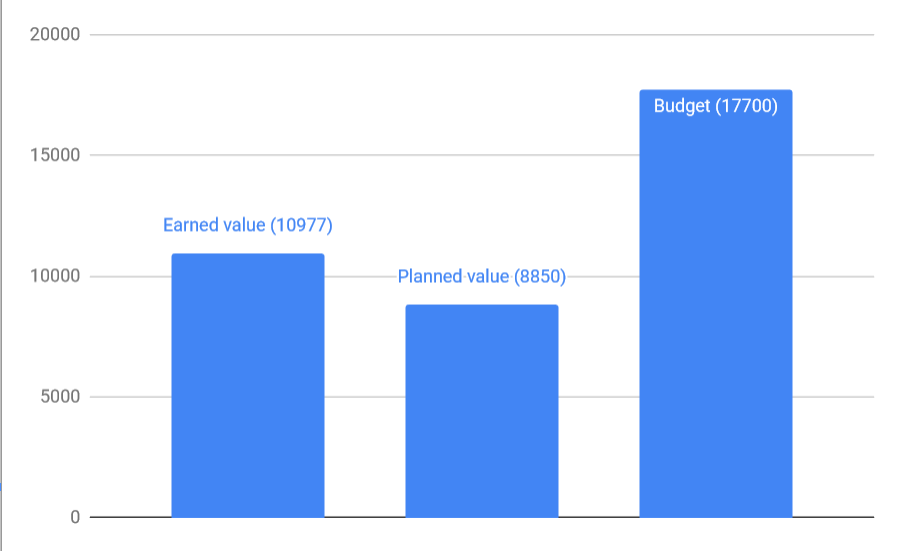
\includegraphics[width=10cm,keepaspectratio]{../includes/pics/SV.PNG}
	\caption{\label{fig:mission}MPRCP001 - Schedule variance}
\end{figure}
\begin{figure}[H]
	\centering
	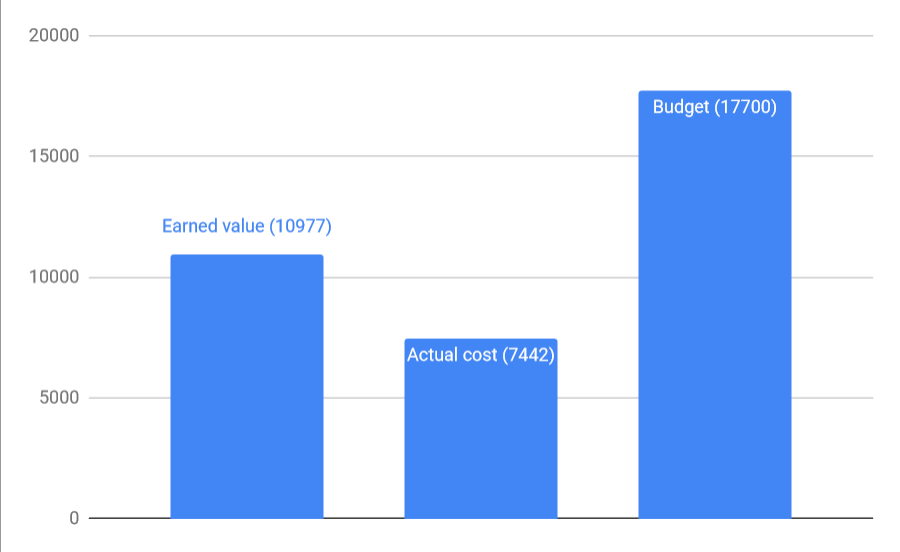
\includegraphics[width=10cm,keepaspectratio]{../includes/pics/BV.PNG}
	\caption{\label{fig:mission}MPRCP002 - Budget variance}
\end{figure}
\paragraph{MPRCP003 - Rischi non previsti}\mbox{}\\[0.4cm]
I rischi presentatisi in questa fase sono tutti già individuati nel set dei rischi. Di conseguenza non viene riportato alcun rischio non preventivato.
\paragraph{MPRCP004 - Indisponibilità servizi terzi}\mbox{}\\[0.4cm]
I servizi terzi utilizzati non hanno subito interruzioni di disponibilità in nessun periodo. Di conseguenza non viene riportata alcuna segnalazione.
\paragraph{MPRCP005 - Media di commit per settimana}\mbox{}\\[0.4cm]
Nella tabella sottostante è mostrato il risultato ottenuto per le repository utilizzate.
\begin{center}%%TODO aggiorna numeri
	\centering
	\renewcommand{\arraystretch}{1.5}
	\rowcolors{3}{tableLightYellow}{}
	\begin{longtable}{  p{5cm}  p{5cm} }
		\rowcolor{tableHeadYellow}
		\textbf{Repository}   & \textbf{N. commit settimanali} \\ 
		\endhead
		Documenti    &           90                      \\
		Applicazione Android         & 9             \\
		Backend AWS    & 20                           \\
		\rowcolor{white}
		\caption{Resoconto misurazioni metrica MPRCP005 - Media commit per settimana}
	\end{longtable}
\end{center}
\pagebreak
\subsubsection{Documenti}
\paragraph{MPRDD001 - Indice di Gulpease}\mbox{}\\[0.4cm]
Per mezzo di script automatici è stato possibile istanziare la metrica  \textbf{MPRDD001 Indice di Gulpease}.\\
Nella tabella sottostante è mostrato il risultato ottenuto per i principali documenti prodotti.
\begin{center}%%TODO aggiorna numeri
	\centering
	\renewcommand{\arraystretch}{1.5}
	\rowcolors{3}{tableLightYellow}{}
	\begin{longtable}{  p{5cm}  p{5cm} p{3cm}  }
		\rowcolor{tableHeadYellow}
		\textbf{Nome documento}   & \textbf{Indice di \mbox{Gulpease}} & \textbf{Esito} \\ 
		\endhead
		Studio di Fattibilità     & 89                                 & Ottimo \\
		Norme di Progetto         & 83                                 & Ottimo \\
		Analisi dei Requisiti     & 81                                 & Ottimo \\
		Piano di Progetto         & 84                                & Ottimo \\
		Piano di Qualifica        & 90                                 & Ottimo \\
		\rowcolor{white}
		\caption{Resoconto misurazioni metrica MPRDD001 - Indice di Gulpease}
	\end{longtable}
\end{center}
\paragraph{MPRDD002 - Errori ortografici}\mbox{}\\[0.4cm]
Tutti i documenti, dopo un rigoroso controllo da parte dei verificatori ed un feedback positivo rilasciato dallo strumento di controllo della sintassi di TexStudio, risultano privi di errori e raggiungono il valore accettabile ed ottimale della metrica  \textbf{MPRDD002 Correttezza ortografica}.
\clearpage
\subsubsection{Software}
\paragraph{MPRDS001 - Copertura requisiti obbligatori}\mbox{}\\[0.4cm]
Sono coperti da implementazione il 62\% dei requisiti obbligatori.
\paragraph{MPRDS002 - Copertura requisiti accettati}\mbox{}\\[0.4cm]
Sono coperti da implementazione il 22\% dei requisiti accettati.
%%ds 4 5 e 6 non sono ancora misurabili
\paragraph{MPRDS009 - Complessità ciclomatica}\mbox{}\\[0.4cm]
La misura è stata effettuata tramite il plugin CodeMR. Per il codice dell' applicazione Android, su un totale di 24 classi, sono state individuate: \begin{itemize}
\item 8 classi di complessità medio-alta (giallo)
\item 7 classi di complessità medio-bassa (verde chiaro) 
\item 6 classi di complessità bassa (verde scuro) 
\end{itemize}
\begin{figure}[H]
	\centering
	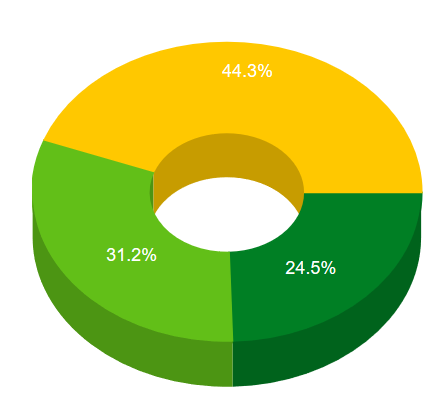
\includegraphics[width=10cm,keepaspectratio]{../includes/pics/complexity.PNG}
	\caption{\label{fig:mission}MPRDS009 - Complessità ciclomatica}
\end{figure}
%%la figura è in pics domani faccio
\paragraph{MPRDS010 - Numero di metodi}\mbox{}\\[0.4cm]
\begin{itemize}
\item La parte Android dell'Applicazione conta di 61 metodi.
\item La parte AWS Lambda dell'Applicazione conta di 30 metodi.
\end{itemize}

%chiedi a chi di competenza 
\paragraph{MPRDS011 - Variabili non utilizzate}\mbox{}\\[0.4cm]
Le variabili inutilizzate sono segnalate come warnings dagli \markg{IDE} utilizzati, sono perciò facili da individuare, il loro valore è 0.
\subsubsection{Test sul software}
I risultati sono relativi allo stato attuale di Revisione di Progettazione, sono stati applicati pochi test per l'applicazione Android, solo quelli necessari a coprire i requisiti necessari ad un proof of concept, per quanto riguarda il backend AWS Lambda i test sono automaticamente generati per ogni Lambda implementata. Non è ancora stato definito il numero totale di test che si andranno ad eseguire.
\paragraph{Test di Unità}
\label{sec:tuRP}
Di seguito vengono riportati i Test di Unità relativi all'applicazione Android realizzata, con descrizione e corrispettivo codice identificativo.
\begin{center}
	\centering
	\renewcommand{\arraystretch}{1.5}
	\rowcolors{3}{tableLightYellow}{}
	\begin{longtable}{  p{1.5cm}  p{10.5cm} p{2cm}  }
		\rowcolor{tableHeadYellow}
		\textbf{Codice}   & \textbf{Descrizione} & \textbf{Esito} \\ 
		\endhead
		TU1 & Verifica che l’utente appena registrato venga salvato nel database.  & Superato \\
		TU2 & Verifica che vengano caricati i workflow dell’utente corrente. & Superato \\
		TU3 & Verifica che il workflow appena creato venga salvato nel database nella giusta forma. & Superato \\
		TU4 & Verifica che vengano caricati i connettori già impostati del workflow selezionato. & Superato \\
		TU5 & Verifica dell’eliminazione dei workflow. & Superato \\
		\rowcolor{white}
		\caption{Elenco Test di Unità}
	\end{longtable}
\end{center}
Per quanto riguarda la Skill sono stati eseguiti i test di unità già forniti da Amazon AWS, restituendo esito positivo per le funzionalità implementate.
\pagebreak
\paragraph{Test di Integrazione}
\label{sec:tiRP}
Di seguito vengono riportati i Test di Integrazione relativi all'applicazione Android realizzata, con descrizione e corrispettivo codice identificativo.
\begin{center}
	\centering
	\renewcommand{\arraystretch}{1.5}
	\rowcolors{3}{tableLightYellow}{}
	\begin{longtable}{  p{1.5cm}  p{10.5cm} p{2cm}  }
		\rowcolor{tableHeadYellow}
		\textbf{Codice}   & \textbf{Descrizione} & \textbf{Esito} \\ 
		\endhead
		TI1 & Verifica la compatibilità tra model view e controller.  & Superato \\
		TI2 & Verifica l’integrazione tra Cognito e DynamoDB. & Superato \\
		TI3 & Verifica l’integrazione tra Skill e DynamoDB. & Superato \\
		\rowcolor{white}
		\caption{Elenco Test di Integrazione}
	\end{longtable}
\end{center}
\paragraph{Test di Sistema}
\label{sec:tsRP}
Di seguito vengono riportati i Test di Sistema relativi all'applicazione Android realizzata, con descrizione e corrispettivo codice identificativo.
\begin{center}
	\centering
	\renewcommand{\arraystretch}{1.5}
	\rowcolors{3}{tableLightYellow}{}
	\begin{longtable}{  p{1.2cm}  p{8.5cm} p{2cm} p{1.5cm} }
		\rowcolor{tableHeadYellow}
		\textbf{Codice}   & \textbf{Descrizione} & \textbf{Cod. \mbox{requisito}} & \textbf{Esito} \\ 
		\endhead
		TS1 & Verifica che il sistema permetta la registrazione. & R2F1 & Superato \\
		TS2 & Verifica che il sistema permetta il login. & R2F2 & Superato \\
		TS3 & Verifica che il sistema permetta l’accesso a tutti i workflow creati dall’utente. & R2F4 & Superato \\
		TS4 & Verifica che il sistema mostri solo i workflow dell’utente corrente. & R2F5 & Superato \\
		TS5 & Verifica che il sistema impedisca la creazione di workflow il cui nome è inferiore ai 4 caratteri. & R2F6 & Superato \\
		TS6 & Verifica che il sistema visualizzi i connettori disponibili. & R2F7 & Superato \\
		\rowcolor{white}
		\caption{Elenco Test di Sistema}
	\end{longtable}
\end{center}
\paragraph{MPRCS006 - Misurazione dei test}
\begin{center}
	\centering
	\renewcommand{\arraystretch}{1.5}
	\rowcolors{3}{tableLightYellow}{}
	\begin{longtable}{  p{5cm}  p{5cm} p{3cm}  }
		\rowcolor{tableHeadYellow}
		\textbf{Metrica}   & \textbf{Valore ottenuto} & \textbf{Esito} \\ 
		\endhead
		Percentuale test passati     & 100\%  & Ottimale \\
		Percentuale test falliti     & 0\% & Ottimale \\
		Efficienza progettazione test    & 25 minuti & Accettabile \\
		Contenimento dei difetti    & 80\% & Accettabile \\
		\rowcolor{white}
		\caption{Resoconto misurazioni metrica MPRCS006 - Misurazione dei test}
	\end{longtable}
\end{center}
\paragraph{MPRCS007 - Copertura requisiti}\mbox{}\\[0.4cm]
In questa revisione la copertura dei requisiti è pari al 63\%, valore considerato non accettato per tale revisione.
Il team terrà in piena considerazione questo risultato per soddisfare a pieno tale metrica per la revisione successiva
\begin{figure}[H]
	\centering
	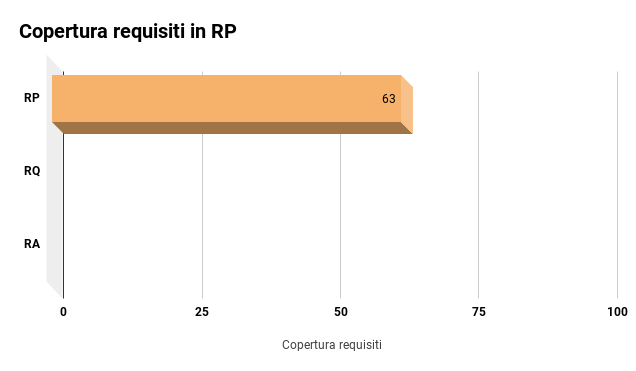
\includegraphics[width=13cm,keepaspectratio]{../includes/pics/CoperturaRP.png}
	\caption{\label{fig:mission}MPRCS007 - Copertura}
\end{figure}

\clearpage
\subsection{Revisione di Qualifica}
\label{sec:revisione_qualifica}
In questa fase del progetto le metriche istanziate saranno quelle di qualità relative ai:
\begin{itemize}
	\item processi;
	\item documenti;
	\item software.
\end{itemize}
\textbf{Attenzione:} Le metriche di qualità per il software utilizzate in questa fase si riferiscono ad un prodotto totalmente finito per la fase di sviluppo. Alcune delle metriche riportate nelle Norme di Progetto v4.0.0 non sono state attuate in quanto alcune di queste servono a qualificare il raffinamento del prodotto.
\subsubsection{Processi}
\paragraph{MPRCP001 - SV e MPRCP002 -  BV}\mbox{}\\[0.4cm]
Schedule variance e budget variance indicano un buono stato di salute del progetto.
\begin{itemize}
	\item SV = +1.150
	\item BV = +1.450
\end{itemize}
\begin{figure}[H]
	\centering
	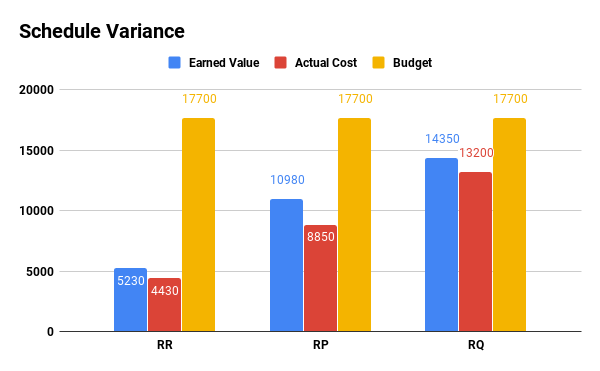
\includegraphics[width=13cm,keepaspectratio]{../includes/pics/Schedule_Variance.png}
	\caption{\label{fig:mission}MPRCP001 - Schedule variance}
\end{figure}
\begin{figure}[H]
	\centering
	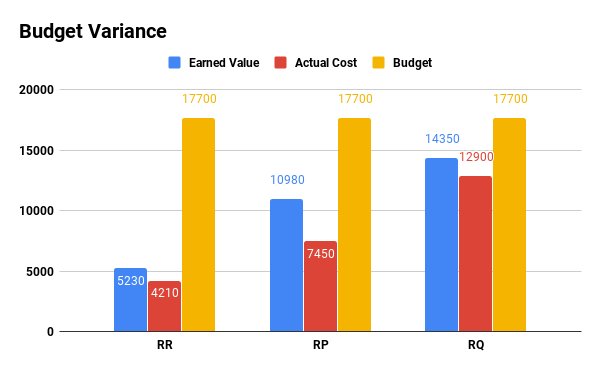
\includegraphics[width=13cm,keepaspectratio]{../includes/pics/Budget_Variance.png}
	\caption{\label{fig:mission}MPRCP002 - Budget variance}
\end{figure}
\paragraph{MPRCP003 - Rischi non previsti}\mbox{}\\[0.4cm]
I rischi presentatisi in questa fase sono tutti già individuati nel set dei rischi. Di conseguenza non viene riportato alcun rischio non preventivato.
\paragraph{MPRCP004 - Indisponibilità servizi terzi}\mbox{}\\[0.4cm]
I servizi terzi utilizzati non hanno subito interruzioni di disponibilità in nessun periodo. Di conseguenza non viene riportata alcuna segnalazione.
\paragraph{MPRCP005 - Media di commit per settimana}\mbox{}\\[0.4cm]
Nella tabella sottostante è mostrato il risultato ottenuto per le repository utilizzate.
\begin{center}%%TODO aggiorna numeri
	\centering
	\renewcommand{\arraystretch}{1.5}
	\rowcolors{3}{tableLightYellow}{}
	\begin{longtable}{  p{5cm}  p{5cm} }
		\rowcolor{tableHeadYellow}
		\textbf{Repository}   & \textbf{N. commit settimanali} \\ 
		\endhead
		Documenti    			   & 84 \\
		Applicazione Android  & 32 \\
		Backend AWS    & 21          \\
		\rowcolor{white}
		\caption{Resoconto misurazioni metrica MPRCP005 - Media commit per settimana}
	\end{longtable}
\end{center}
\begin{figure}[H]
	\centering
	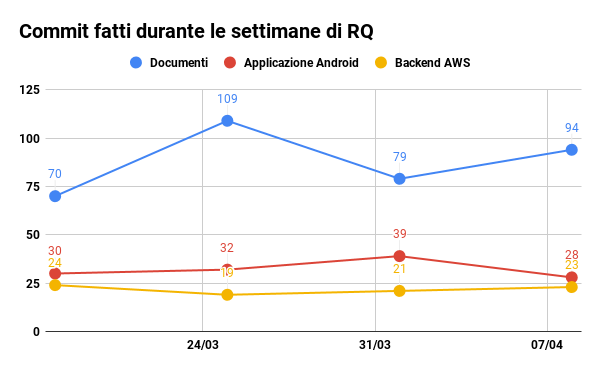
\includegraphics[width=13cm,keepaspectratio]{../includes/pics/Commit_RQ.png}
	\caption{\label{fig:mission}MPRCP005 - Commit fatti durante le settimane di RQ}
\end{figure}
\subsubsection{Documenti}
\paragraph{MPRDD001 - Indice di Gulpease}\mbox{}\\[0.4cm]
Per mezzo di script automatici è stato possibile istanziare la metrica  \textbf{MPRDD001 Indice di Gulpease}.\\
Nella tabella sottostante è mostrato il risultato ottenuto per i principali documenti prodotti.
\begin{center}%%TODO aggiorna numeri
	\centering
	\renewcommand{\arraystretch}{1.5}
	\rowcolors{3}{tableLightYellow}{}
	\begin{longtable}{  p{5cm}  p{5cm} p{3cm}  }
		\rowcolor{tableHeadYellow}
		\textbf{Nome documento}   & \textbf{Indice di \mbox{Gulpease}} & \textbf{Esito} \\ 
		\endhead
		Norme di Progetto         & 81                                 & Ottimo \\
		Analisi dei Requisiti     & 83                                 & Ottimo \\
		Piano di Progetto         & 87                                & Ottimo \\
		Piano di Qualifica        & 87                                 & Ottimo \\
		Manuale Utente  	& 88 & Ottimo \\
		Manuale Programmatore & 81 & Ottimo \\
		\rowcolor{white}
		\caption{Resoconto misurazioni metrica MPRDD001 - Indice di Gulpease}
	\end{longtable}
	\begin{figure}[H]
		\centering
		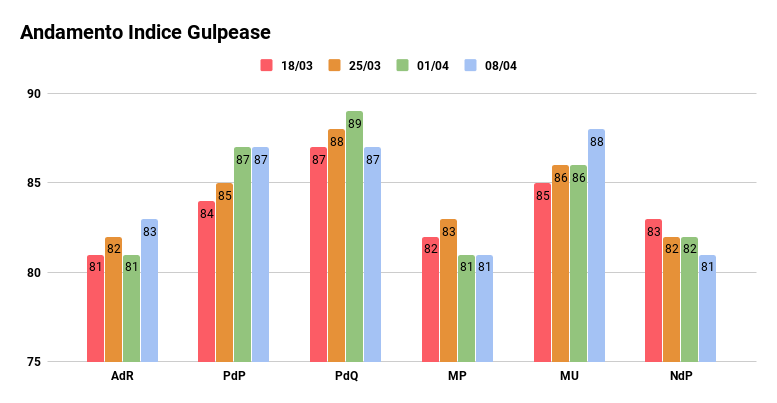
\includegraphics[width=13cm,keepaspectratio]{../includes/pics/Gulpease.png}
		\caption{\label{fig:mission}MPRDD001 - Grafico andamento Indice di Gulpease in RQ}
	\end{figure}
\end{center}
\paragraph{MPRDD002 - Errori ortografici}\mbox{}\\[0.4cm]
Tutti i documenti, dopo un rigoroso controllo da parte dei verificatori ed un feedback positivo rilasciato dallo strumento di controllo della sintassi di TexStudio, risultano privi di errori e raggiungono il valore accettabile ed ottimale della metrica  \textbf{MPRDD002 Correttezza ortografica}.
\begin{figure}[H]
	\centering
	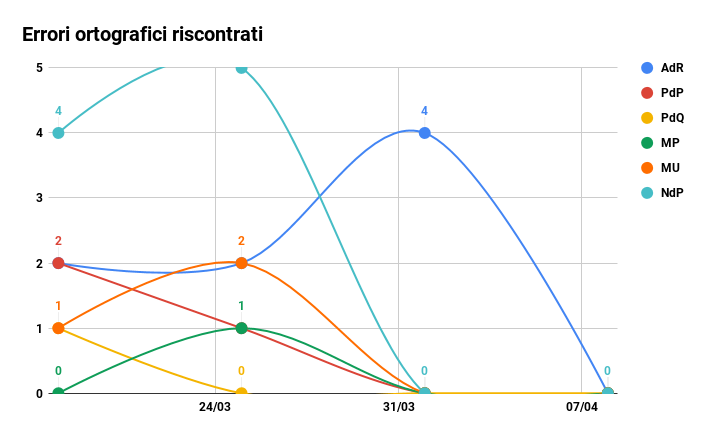
\includegraphics[width=13cm,keepaspectratio]{../includes/pics/Errori.png}
	\caption{\label{fig:mission}MPRDD002 - Grafico Errori ortografici riscontrati in RQ}
\end{figure}
\clearpage
\subsubsection{Software}
\paragraph{MPRDS001 - Copertura requisiti obbligatori}\mbox{}\\[0.4cm]
Sono coperti da implementazione il 83\% dei requisiti obbligatori.
\paragraph{MPRDS002 - Copertura requisiti accettati}\mbox{}\\[0.4cm]
Sono coperti da implementazione il 32\% dei requisiti accettati.
\begin{figure}[H]
	\centering
	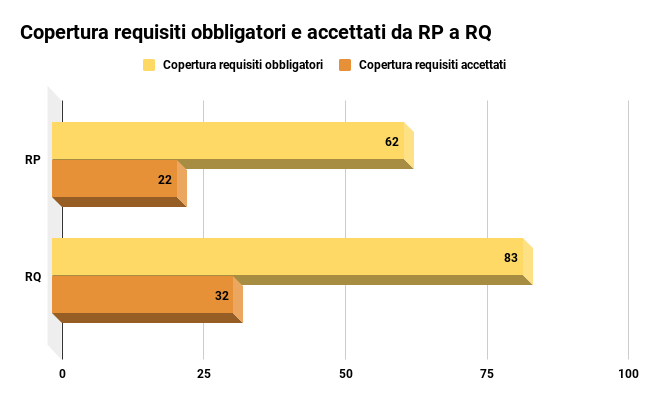
\includegraphics[width=13cm,keepaspectratio]{../includes/pics/Copertura.png}
	\caption{\label{fig:mission}MPRDS001 e MPRDS002 - Copertura requisiti obbligatori e Copertura requisiti accettati in RQ}
\end{figure}
\paragraph{MPRDS009 - Complessità ciclomatica}\mbox{}\\[0.4cm]
La misura è stata effettuata tramite il plugin CodeMR. Per il codice dell' applicazione Android, su un totale di 16 classi, sono state individuate: \begin{itemize}
	\item 5 classi di complessità medio-alta(giallo)
	\item 4 classi di complessità medio-bassa (verde chiaro)
	\item 2 classi di complessità bassa (verde scuro)
\end{itemize}
\begin{figure}[H]
	\centering
	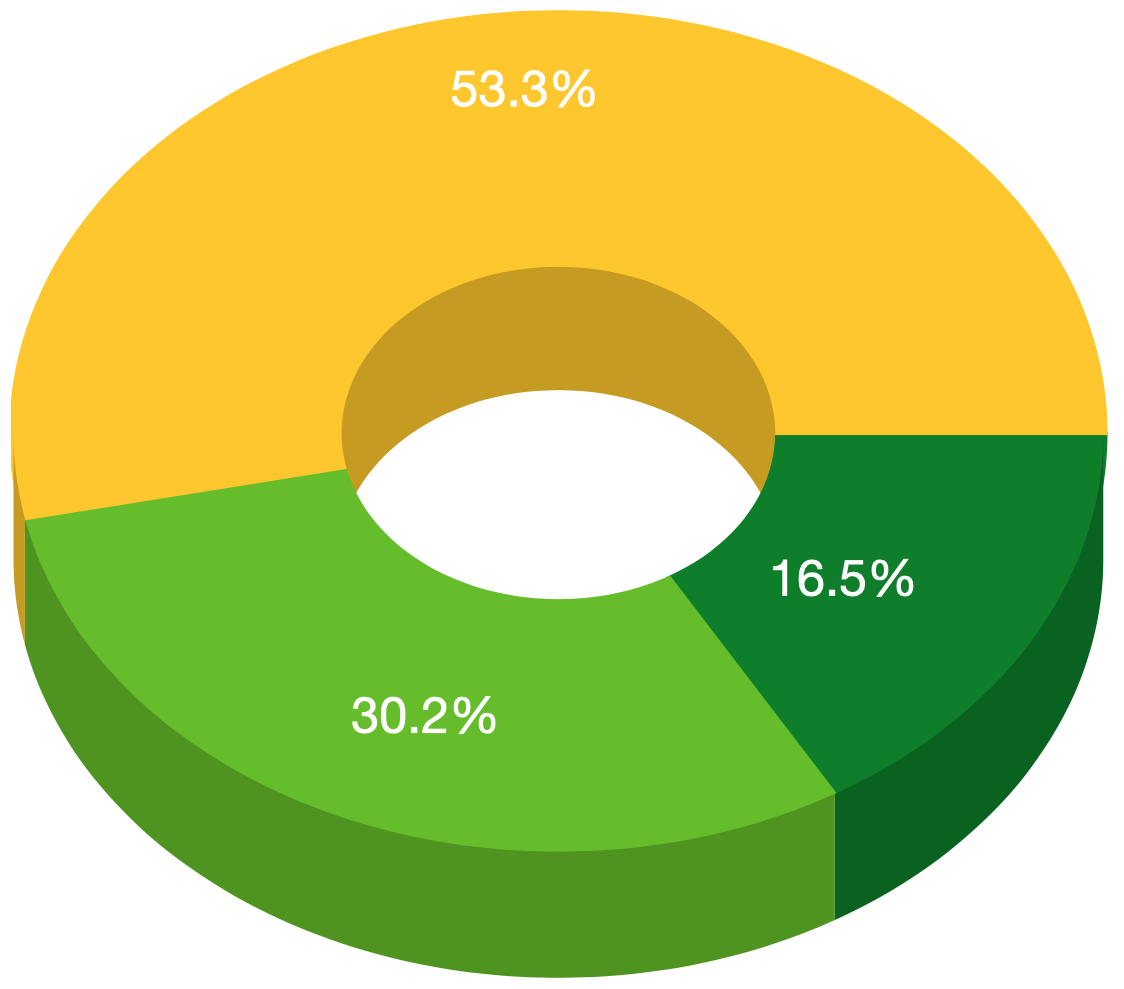
\includegraphics[width=10cm,keepaspectratio]{../includes/pics/complex.png}
	\caption{\label{fig:mission}MPRDS009 - Complessità ciclomatica}
\end{figure}
\paragraph{MPRDS010 - Numero di metodi}
\begin{itemize}
	\item La parte Android dell'Applicazione conta di 49 metodi.
	\item La parte AWS Lambda dell'Applicazione conta di 40 metodi.
\end{itemize}
\begin{figure}[H]
	\centering
	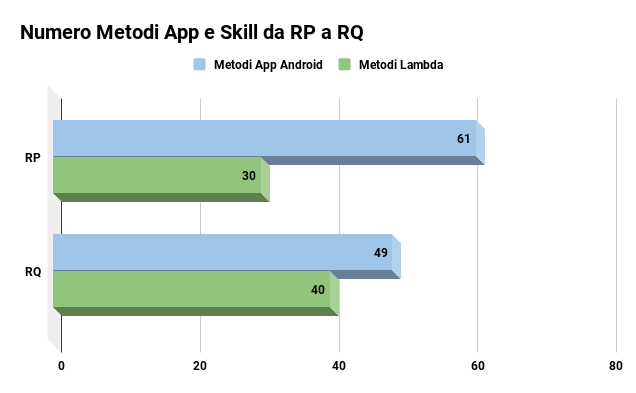
\includegraphics[width=13cm,keepaspectratio]{../includes/pics/nMetodi.png}
	\caption{\label{fig:mission}MPRDS010 -  Numero di metodi da RP a RQ}
\end{figure}
Notiamo dal grafico sopra riportato che il numero di metodi sia per l'applicazione Android sia per le funzioni AWS Lambda è diminuito, questo perché tante funzionalità sono state migliorate appoggiandosi ai servizi e alle funzioni di Amazon AWS, snellendo così il codice e migliorandone l'efficienza e l'efficacia.
\paragraph{MPRDS011 - Variabili non utilizzate}\mbox{}\\[0.4cm]
Le variabili inutilizzate sono segnalate come warnings dagli \markg{IDE} utilizzati, sono perciò facili da individuare, il loro valore è 0.
\subsubsection{Test sul software}
I risultati sono relativi allo stato attuale di Revisione di Qualifica. Sono stati applicati i test necessari a coprire i requisiti obbligatori di qualità sui prodotti. Per l'app Android sono stati applicati test per verificare le funzionalità dei metodi, mentre per quanto riguarda il backend della Skill i test sono automaticamente generati per ogni funzione Lambda implementata. Non è ancora stato definito il numero totale di test che si andranno ad eseguire.
\paragraph{Test di Unità}
\label{sec:tuRQ}
Di seguito vengono riportati i Test di Unità relativi all'applicazione Android realizzata, con descrizione e corrispettivo codice identificativo.
\begin{center}
	\centering
	\renewcommand{\arraystretch}{1.5}
	\rowcolors{3}{tableLightYellow}{}
	\begin{longtable}{  p{1.5cm}  p{10.5cm} p{2cm}  }
		\rowcolor{tableHeadYellow}
		\textbf{Codice}   & \textbf{Descrizione} & \textbf{Esito} \\ 
		\endhead
		TU1 & Verifica che l’utente appena registrato venga salvato nel database.  & Superato \\
		TU2 & Verifica che vengano caricati i workflow dell’utente corrente. & Superato \\
		TU3 & Verifica che il workflow appena creato venga salvato nel database nella giusta forma. & Superato \\
		TU4 & Verifica che vengano caricati i connettori già impostati del workflow selezionato. & Superato \\
		TU5 & Verifica dell’eliminazione dei workflow. & Superato \\
		TU6 & Verifica che vengano caricati i parametri già impostati dei connettori già impostati del workflow selezionato. & Superato \\
		\rowcolor{white}
		\caption{Elenco Test di Unità}
	\end{longtable}
\end{center}
Per quanto riguarda la Skill sono stati eseguiti i test di unità già forniti da Amazon AWS, restituendo esito positivo per le funzionalità implementate.
\paragraph{Test di Integrazione}
\label{sec:tiRQ}
Di seguito vengono riportati i Test di Integrazione relativi all'applicazione Android realizzata, con descrizione e corrispettivo codice identificativo.
\begin{center}
	\centering
	\renewcommand{\arraystretch}{1.5}
	\rowcolors{3}{tableLightYellow}{}
	\begin{longtable}{  p{1.5cm}  p{10.5cm} p{2cm}  }
		\rowcolor{tableHeadYellow}
		\textbf{Codice}   & \textbf{Descrizione} & \textbf{Esito} \\ 
		\endhead
		TI1 & Verifica la compatibilità tra model view e controller.  & Superato \\
		TI2 & Verifica l’integrazione tra Cognito e DynamoDB. & Superato \\
		TI3 & Verifica l’integrazione tra Skill e DynamoDB. & Superato \\
		TI4 & Verifica l’integrazione tra AWS MobileClient e Cognito. & Superato \\
		TI5 & Verifica integrazione tra GraphQL Schema e AppSync. & Superato \\
		\rowcolor{white}
		\caption{Elenco Test di Integrazione}
	\end{longtable}
\end{center}
\paragraph{Test di Sistema}
\label{sec:tsRQ}
Di seguito vengono riportati i Test di Sistema relativi all'applicazione Android realizzata, con descrizione e corrispettivo codice identificativo.
\begin{center}
	\centering
	\renewcommand{\arraystretch}{1.5}
	\rowcolors{3}{tableLightYellow}{}
	\begin{longtable}{  p{1.2cm}  p{8.5cm} p{2cm} p{1.5cm} }
		\rowcolor{tableHeadYellow}
		\textbf{Codice}   & \textbf{Descrizione} & \textbf{Cod. \mbox{requisito}} & \textbf{Esito} \\ 
		\endhead
		TS1 & Verifica che il sistema permetta la registrazione. & R2F1 & Superato \\
		TS2 & Verifica che il sistema permetta il login. & R2F2 & Superato \\
		TS3 & Verifica che il sistema permetta l’accesso a tutti i workflow creati dall’utente. & R2F4 & Superato \\
		TS4 & Verifica che il sistema mostri solo i workflow dell’utente corrente. & R2F5 & Superato \\
		TS5 & Verifica che il sistema impedisca la creazione di workflow il cui nome è inferiore ai 4 caratteri. & R2F6 & Superato \\
		TS6 & Verifica che il sistema visualizzi i connettori disponibili. & R2F7 & Superato \\
		\rowcolor{white}
		\caption{Elenco Test di Sistema}
	\end{longtable}
\end{center}
\pagebreak
\paragraph{MPRCS006 - Misurazione dei test}
\begin{center}
	\centering
	\renewcommand{\arraystretch}{1.5}
	\rowcolors{3}{tableLightYellow}{}
	\begin{longtable}{  p{5cm}  p{5cm} p{3cm}  }
		\rowcolor{tableHeadYellow}
		\textbf{Metrica}   & \textbf{Valore ottenuto} & \textbf{Esito} \\ 
		\endhead
		Percentuale test passati     & 100\%  & Ottimale \\
		Percentuale test falliti     & 0\% & Ottimale \\
		Efficienza progettazione test    & 15 minuti & Accettabile \\
		Contenimento dei difetti    & 91\% & Accettabile \\
		\rowcolor{white}
		\caption{Resoconto misurazioni metrica MPRCS006 - Misurazione dei test}
	\end{longtable}
\end{center}
\begin{figure}[H]
	\centering
	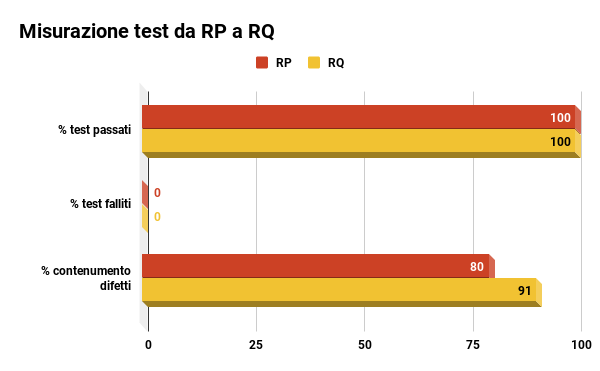
\includegraphics[width=13cm,keepaspectratio]{../includes/pics/Misurazione.png}
	\caption{\label{fig:mission}MPRCS006 - Misurazione dei test da RP a RQ}
\end{figure}
\pagebreak
\paragraph{MPRCS007 - Copertura requisiti}\mbox{}\\[0.4cm]
In questa revisione la copertura dei requisiti è pari al 73\%, valore considerato accettato per tale revisione.
\begin{figure}[H]
	\centering
	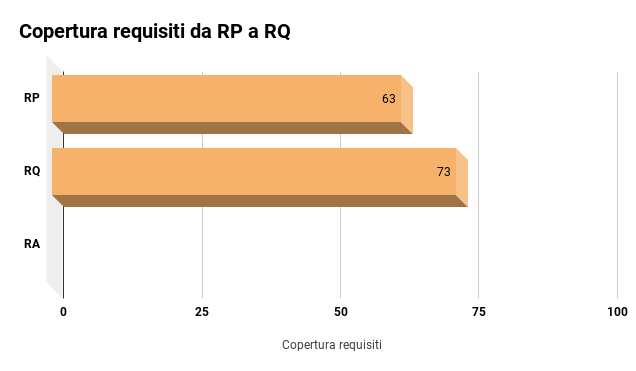
\includegraphics[width=13cm,keepaspectratio]{../includes/pics/CoperturaRP_RQ.png}
	\caption{\label{fig:mission}MPRCS007 - Copertura}
\end{figure}
\paragraph{MPRDS014 - Code Coverage}\mbox{}\\[0.4cm]
\label{sec:CCRQ}
In questa revisione il Code Coverage calcolato è pari al 91\%, valore considerato accettato per tale revisione.
\begin{figure}[H]
	\centering
	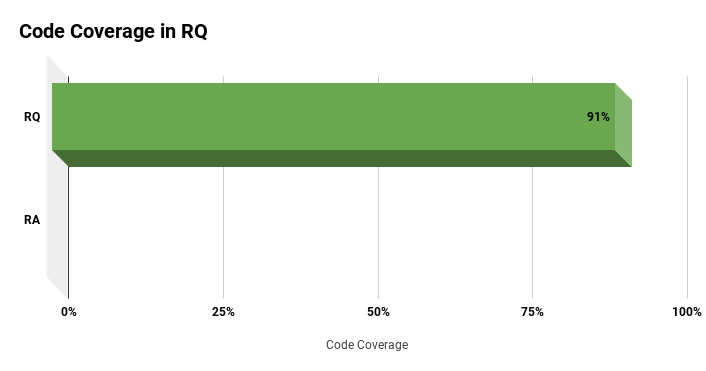
\includegraphics[width=13cm,keepaspectratio]{../includes/pics/ccRQ.png}
	\caption{\label{fig:mission}MPRDS014 - Code Coverage}
\end{figure}

\clearpage
\subsection{Revisione di Accettazione}
\label{sec:revisione_accettazione}
In questa fase del progetto le metriche istanziate saranno quelle di qualità relative ai:
\begin{itemize}
	\item processi;
	\item documenti;
	\item software.
\end{itemize}
\textbf{Attenzione:} Le metriche di qualità per il software utilizzate in questa fase si riferiscono ad un prodotto totalmente finito per la fase di sviluppo. Alcune delle metriche riportate nelle Norme di Progetto v4.0.0 non sono state attuate in quanto alcune di queste servono a qualificare il raffinamento del prodotto.
\subsubsection{Processi}
\paragraph{MPRCP001 - SV e MPRCP002 -  BV}\mbox{}\\[0.4cm]
Schedule variance e budget variance indicano un buono stato di salute del progetto.
\begin{itemize}
	\item SV = + 160
	\item BV = + 500
\end{itemize}
\begin{figure}[H]
	\centering
	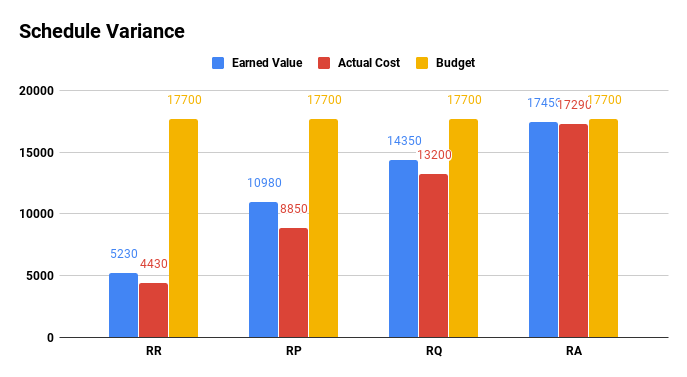
\includegraphics[width=13cm,keepaspectratio]{../includes/pics/Schedule_VarianceRA.png}
	\caption{\label{fig:mission}MPRCP001 - Schedule variance}
\end{figure}
\begin{figure}[H]
	\centering
	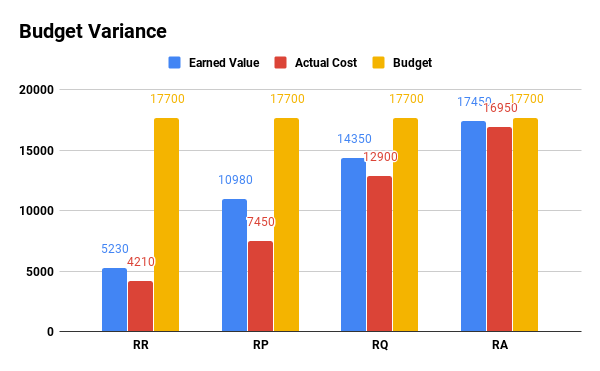
\includegraphics[width=13cm,keepaspectratio]{../includes/pics/Budget_VarianceRA.png}
	\caption{\label{fig:mission}MPRCP002 - Budget variance}
\end{figure}
\paragraph{MPRCP003 - Rischi non previsti}\mbox{}\\[0.4cm]
I rischi presentatisi in questa fase sono tutti già individuati nel set dei rischi. Di conseguenza non viene riportato alcun rischio non preventivato.
\paragraph{MPRCP004 - Indisponibilità servizi terzi}\mbox{}\\[0.4cm]
I servizi terzi utilizzati non hanno subito interruzioni di disponibilità in nessun periodo. Di conseguenza non viene riportata alcuna segnalazione.
\paragraph{MPRCP005 - Media di commit per settimana}\mbox{}\\[0.4cm]
Nella tabella sottostante è mostrato il risultato ottenuto per le repository utilizzate.
\begin{center}
	\centering
	\renewcommand{\arraystretch}{1.5}
	\rowcolors{3}{tableLightYellow}{}
	\begin{longtable}{  p{5cm}  p{5cm} }
		\rowcolor{tableHeadYellow}
		\textbf{Repository}   & \textbf{N. commit settimanali} \\ 
		\endhead
		Documenti    			   & 72 \\
		Applicazione Android  & 37 \\
		Backend AWS    & 29          \\
		\rowcolor{white}
		\caption{Resoconto misurazioni metrica MPRCP005 - Media commit per settimana}
	\end{longtable}
\end{center}
\begin{figure}[H]
	\centering
	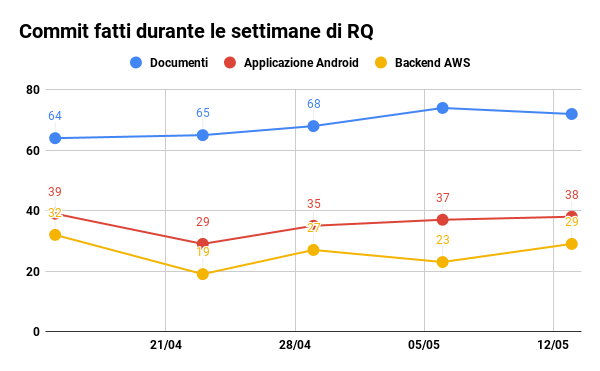
\includegraphics[width=13cm,keepaspectratio]{../includes/pics/Commit_RA.png}
	\caption{\label{fig:mission}MPRCP005 - Commit fatti durante le settimane di RA}
\end{figure}
\subsubsection{Documenti}
\paragraph{MPRDD001 - Indice di Gulpease}\mbox{}\\[0.4cm]
Per mezzo di script automatici è stato possibile istanziare la metrica  \textbf{MPRDD001 Indice di Gulpease}.\\
Nella tabella sottostante è mostrato il risultato ottenuto per i principali documenti prodotti.
\begin{center}%%TODO aggiorna numeri
	\centering
	\renewcommand{\arraystretch}{1.5}
	\rowcolors{3}{tableLightYellow}{}
	\begin{longtable}{  p{5cm}  p{5cm} p{3cm}  }
		\rowcolor{tableHeadYellow}
		\textbf{Nome documento}   & \textbf{Indice di \mbox{Gulpease}} & \textbf{Esito} \\ 
		\endhead
		Norme di Progetto         & 81                                 & Ottimo \\
		Analisi dei Requisiti     & 83                                 & Ottimo \\
		Piano di Progetto         & 87                                & Ottimo \\
		Piano di Qualifica        & 93                                 & Ottimo \\
		Manuale Utente  	& 92 & Ottimo \\
		Manuale Programmatore & 83 & Ottimo \\
		\rowcolor{white}
		\caption{Resoconto misurazioni metrica MPRDD001 - Indice di Gulpease}
	\end{longtable}
	\begin{figure}[H]
		\centering
		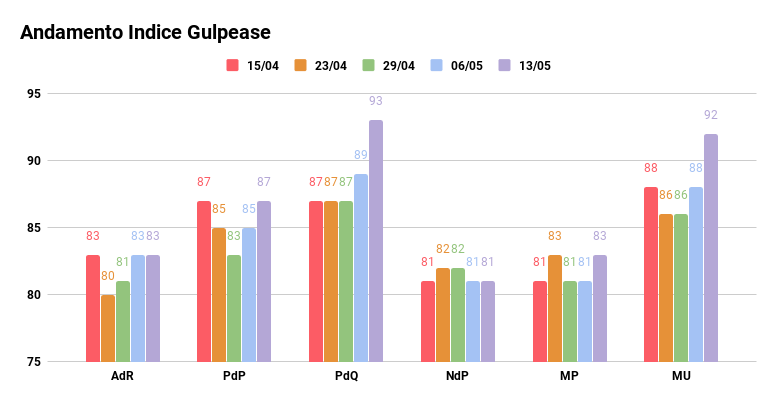
\includegraphics[width=13cm,keepaspectratio]{../includes/pics/Indice_GulpeaseRA.png}
		\caption{\label{fig:mission}MPRDD001 - Grafico andamento Indice di Gulpease in RA}
	\end{figure}
\end{center}
\paragraph{MPRDD002 - Errori ortografici}\mbox{}\\[0.4cm]
Tutti i documenti, dopo un rigoroso controllo da parte dei verificatori ed un feedback positivo rilasciato dallo strumento di controllo della sintassi di TexStudio, risultano privi di errori e raggiungono il valore accettabile ed ottimale della metrica  \textbf{MPRDD002 Correttezza ortografica}.
\begin{figure}[H]
	\centering
	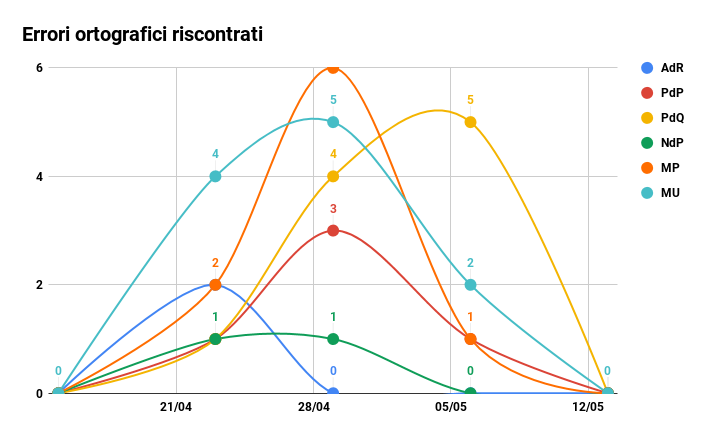
\includegraphics[width=13cm,keepaspectratio]{../includes/pics/ErroriRA.png}
	\caption{\label{fig:mission}MPRDD002 - Grafico Errori ortografici riscontrati in RQ}
\end{figure}
\clearpage
\subsubsection{Software}
\paragraph{MPRDS001 - Copertura requisiti obbligatori}\mbox{}\\[0.4cm]
Sono coperti da implementazione il 100\% dei requisiti obbligatori.
\paragraph{MPRDS002 - Copertura requisiti accettati}\mbox{}\\[0.4cm]
Sono coperti da implementazione il 63\% dei requisiti accettati.
\begin{figure}[H]
	\centering
	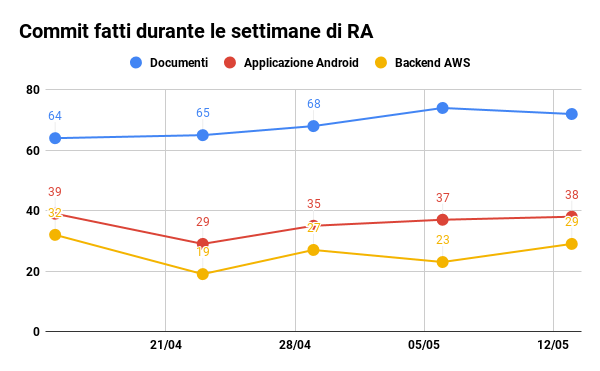
\includegraphics[width=13cm,keepaspectratio]{../includes/pics/CoperturaRA.png}
	\caption{\label{fig:mission}MPRDS001 e MPRDS002 - Copertura requisiti obbligatori e Copertura requisiti accettati in RA}
\end{figure}
\paragraph{MPRDS009 - Complessità ciclomatica}\mbox{}\\[0.4cm]
La misura è stata effettuata tramite il plugin CodeMR. Per il codice dell' applicazione Android, su un totale di 16 classi, sono state individuate: \begin{itemize}
	\item 5 classi di complessità medio-alta (giallo)
	\item 4 classi di complessità medio-bassa (verde chiaro)
	\item 2 classi di complessità bassa (verde scuro)
\end{itemize}
\begin{figure}[H]
	\centering
	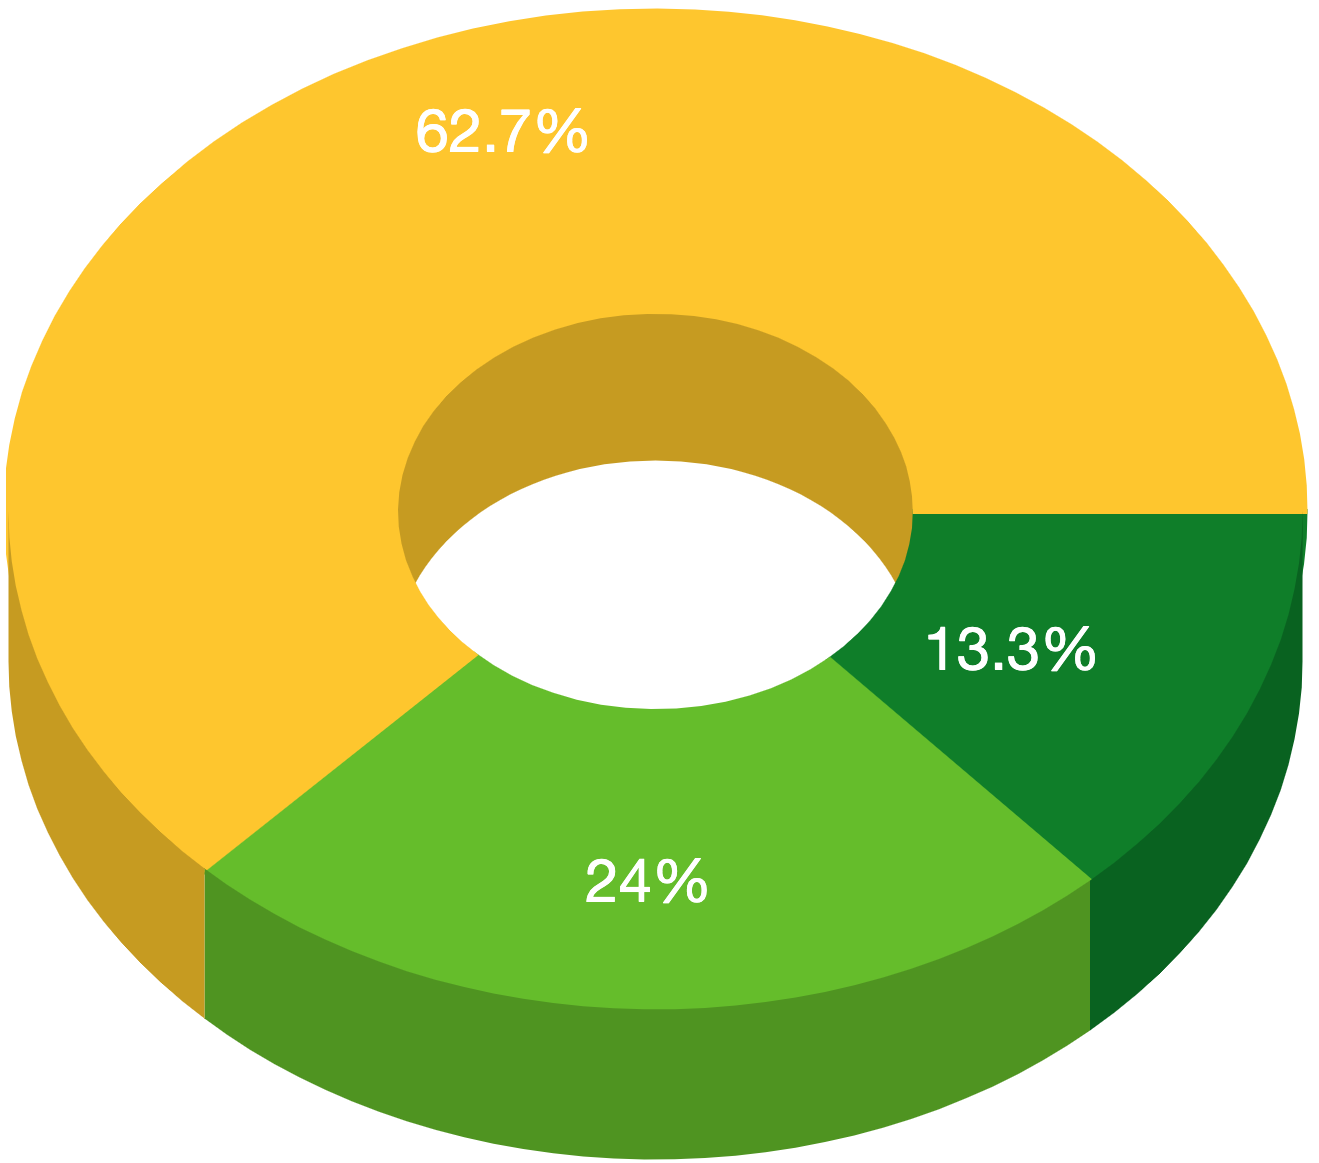
\includegraphics[width=10cm,keepaspectratio]{../includes/pics/complexRA.png}
	\caption{\label{fig:mission}MPRDS009 - Complessità ciclomatica}
\end{figure}
Di seguito viene riportato l'andamento della Complessità Ciclomatica del prodotto software nella fase da Revisione di Progettazione a Revisione di Accettazione:
\begin{figure}[H]
	\centering
	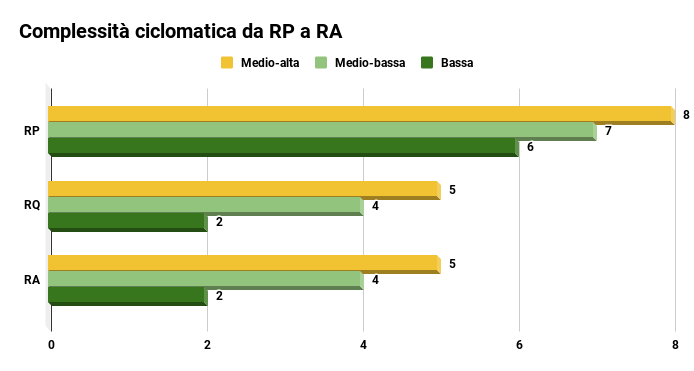
\includegraphics[width=13cm,keepaspectratio]{../includes/pics/complexCiclo.png}
	\caption{\label{fig:mission}MPRDS009 - Complessità ciclomatica da RP a RA}
\end{figure}
\paragraph{MPRDS010 - Numero di metodi}
\begin{itemize}
	\item La parte Android dell'Applicazione conta di 49 metodi.
	\item La parte AWS Lambda dell'Applicazione conta di 40 metodi.
\end{itemize}
\begin{figure}[H]
	\centering
	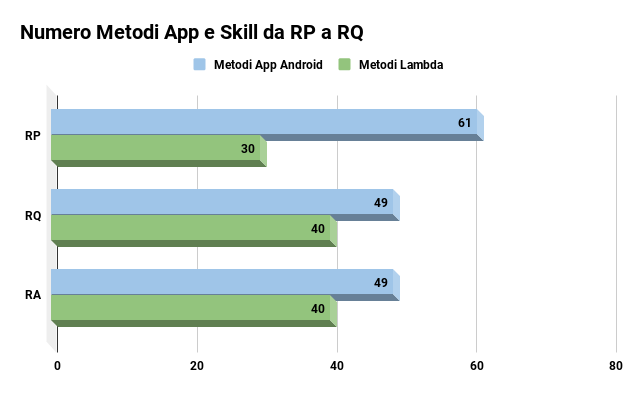
\includegraphics[width=13cm,keepaspectratio]{../includes/pics/nMetodiRA.png}
	\caption{\label{fig:mission}MPRDS010 -  Numero di metodi da RP a RA}
\end{figure}
Notiamo dal grafico sopra riportato che il numero di metodi sia per l'applicazione Android sia per le funzioni AWS Lambda è rimasto costante dalla Revisione precedente, questo perché le funzionalità sono già state implementate migliorate appoggiandosi ai servizi, alle funzioni di Amazon AWS e ai Design Pattern adottati.
\paragraph{MPRDS011 - Variabili non utilizzate}\mbox{}\\[0.4cm]
Le variabili inutilizzate sono segnalate come warnings dagli \markg{IDE} utilizzati, sono perciò facili da individuare, il loro valore è 0.
\subsubsection{Test sul software}
I risultati sono relativi allo stato di Revisione di Accettazione. Sono stati applicati i test necessari a coprire i requisiti obbligatori di qualità sui prodotti. Per l'app Android sono stati applicati test per verificare le funzionalità dei metodi, mentre per quanto riguarda il backend della Skill i test sono automaticamente generati per ogni funzione Lambda implementata.
\pagebreak
\paragraph{Test di Unità}
\label{sec:tuRA}
Di seguito vengono riportati i Test di Unità relativi all'applicazione Android realizzata, con descrizione e corrispettivo codice identificativo.
\begin{center}
	\centering
	\renewcommand{\arraystretch}{1.5}
	\rowcolors{3}{tableLightYellow}{}
	\begin{longtable}{  p{1.5cm}  p{10.5cm} p{2cm}  }
		\rowcolor{tableHeadYellow}
		\textbf{Codice}   & \textbf{Descrizione} & \textbf{Esito} \\ 
		\endhead
		TU1 & Verifica che l’utente appena registrato venga salvato nel database.  & Superato \\
		TU2 & Verifica che vengano caricati i workflow dell’utente corrente. & Superato \\
		TU3 & Verifica che il workflow appena creato venga salvato nel database nella giusta forma. & Superato \\
		TU4 & Verifica che vengano caricati i connettori già impostati del workflow selezionato. & Superato \\
		TU5 & Verifica dell’eliminazione dei workflow. & Superato \\
		TU6 & Verifica che vengano caricati i parametri già impostati dei connettori già impostati del workflow selezionato. & Superato \\
		TU7 & Verifica che salvando i connettori appena aggiunti e impostati questi vengano aggiunti nel DB nella corretta forma. & Superato \\
		TU8 & Verifica dell’eliminazione dei connettori. & Superato \\
		\rowcolor{white}
		\caption{Elenco Test di Unità}
	\end{longtable}
\end{center}
Per quanto riguarda la Skill sono stati eseguiti i test di unità già forniti da Amazon AWS, restituendo esito positivo per le funzionalità implementate.
\paragraph{Test di Integrazione}
\label{sec:tiRA}
Di seguito vengono riportati i Test di Integrazione relativi all'applicazione Android realizzata, con descrizione e corrispettivo codice identificativo.
\begin{center}
	\centering
	\renewcommand{\arraystretch}{1.5}
	\rowcolors{3}{tableLightYellow}{}
	\begin{longtable}{  p{1.5cm}  p{10.5cm} p{2cm}  }
		\rowcolor{tableHeadYellow}
		\textbf{Codice}   & \textbf{Descrizione} & \textbf{Esito} \\ 
		\endhead
		TI1 & Verifica la compatibilità tra model view e controller.  & Superato \\
		TI2 & Verifica l’integrazione tra Cognito e DynamoDB. & Superato \\
		TI3 & Verifica l’integrazione tra Skill e DynamoDB. & Superato \\
		TI4 & Verifica l’integrazione tra AWS MobileClient e Cognito. & Superato \\
		TI5 & Verifica integrazione tra GraphQL Schema e AppSync. & Superato \\
		\rowcolor{white}
		\caption{Elenco Test di Integrazione}
	\end{longtable}
\end{center}
\paragraph{Test di Sistema}
\label{sec:tsRA}
Di seguito vengono riportati i Test di Sistema relativi all'applicazione Android realizzata, con descrizione e corrispettivo codice identificativo.
\begin{center}
	\centering
	\renewcommand{\arraystretch}{1.5}
	\rowcolors{3}{tableLightYellow}{}
	\begin{longtable}{  p{1.2cm}  p{8.5cm} p{2cm} p{1.5cm} }
		\rowcolor{tableHeadYellow}
		\textbf{Codice}   & \textbf{Descrizione} & \textbf{Cod. \mbox{requisito}} & \textbf{Esito} \\ 
		\endhead
		TS1 & Verifica che il sistema permetta la registrazione. & R2F1 & Superato \\
		TS2 & Verifica che il sistema permetta il login. & R2F2 & Superato \\
		TS3 & Verifica che il sistema permetta l’accesso a tutti i workflow creati dall’utente. & R2F4 & Superato \\
		TS4 & Verifica che il sistema mostri solo i workflow dell’utente corrente. & R2F5 & Superato \\
		TS5 & Verifica che il sistema impedisca la creazione di workflow il cui nome è inferiore ai 4 caratteri. & R2F6 & Superato \\
		TS6 & Verifica che il sistema visualizzi i connettori disponibili. & R2F7 & Superato \\
		\rowcolor{white}
		\caption{Elenco Test di Sistema}
	\end{longtable}
\end{center}
\pagebreak
\paragraph{Test di Validazione}
\label{sec:tvRA}
Di seguito vengono riportati i Test di Validazione relativi all'applicazione Android realizzata, con descrizione e corrispettivo codice identificativo, che andranno eseguiti in sede ufficiale in presenza di \textit{Zero12.}
\begin{center}
	\centering
	\renewcommand{\arraystretch}{1.5}
	\rowcolors{3}{tableLightYellow}{}
	\begin{longtable}{  p{1.2cm}  p{8cm} p{1.8cm} p{2.2cm} }
		\rowcolor{tableHeadYellow}
		\textbf{Codice}   & \textbf{Descrizione} & \textbf{Cod. \mbox{requisito}} & \textbf{Esito} \\ 
		\endhead
		TV1 & Verificare che il sistema permetta di registrarsi creando un area personale nella quale inserire workflow. & R2F1 & Non \mbox{implementato} \\
		TV2 & Verificare che il sistema permetta il login. & R2F2 & Non \mbox{implementato} \\
		TV3 & Verificare che il sistema non permetta l’inserimento di workflow con nome di meno di 4 caratteri. & R2F6 & Non \mbox{implementato} \\
		TV4 & Verificare che il sistema mostri i connettori disponibili. & R2F7 & Non \mbox{implementato} \\
		TV5 & Verificare che il sistema permetta di avviare il workflow tramite comando vocale impartito ad Alexa. & R2F9 & Non \mbox{implementato} \\
		TV6 & Verificare che il sistema permetta di fermare l’esecuzione vocale del workflow tramite comando vocale ad alexa. & R2F12 & Non \mbox{implementato} \\
		\rowcolor{white}
		\caption{Elenco Test di Validazione}
	\end{longtable}
\end{center}
Di seguito vengono descritte le procedure di attuazione dei Test di Validazione sopra riportate.
\begin{center}
	\centering
	\renewcommand{\arraystretch}{1.5}
	\rowcolors{3}{tableLightYellow}{}
	\begin{longtable}{  p{1.5cm}  p{12.5cm} }
		\rowcolor{tableHeadYellow}
		\textbf{Codice}   & \textbf{Procedura}  \\ 
		\endhead		
		TV1 & L’utente inserisce i dati per la registrazione e conferma i dati. Inserisce il codice arrivatogli per mail per completare la registrazione. Arriva ad una bacheca vuota dove può inserire e visualizzare i workflow inseriti. \\
		TV2 & L’utente inserisce i dati per il login e conferma i dati. L’utente arriva nella sua area personale e visualizza i workflow creati in precedenza se presenti. \\
		TV3 & L’utente prova a inserire un workflow con nome di meno di 4 caratteri. Il sistema avvisa l'utente che non è permesso e non salva il workflow. \\
		TV4 & L’utente crea un workflow e preme il bottone per impostarlo. Il sistema presenta all’utente una lista dei connettori disponibili. \\
		TV5 & L’utente comunica ad Alexa di voler avviare la skill. Alexa chiede che workflow avviare. L’utente comunica il nome del workflow Se valido e presente Alexa avvia le azioni del Workflow. \\
		TV6 & Alexa sta eseguendo un workflow. L’utente impartisce un comando di stop all’assistente vocale (“stop” o “fermati”). L’assistente vocale interrompe l’esecuzione e chiede la prossima azione da eseguire. \\
		\rowcolor{white}
		\caption{Elenco procedure Test di Integrazione}
	\end{longtable}
\end{center}
\pagebreak
\paragraph{MPRCS006 - Misurazione dei test}
\begin{center}
	\centering
	\renewcommand{\arraystretch}{1.5}
	\rowcolors{3}{tableLightYellow}{}
	\begin{longtable}{  p{5cm}  p{5cm} p{3cm}  }
		\rowcolor{tableHeadYellow}
		\textbf{Metrica}   & \textbf{Valore ottenuto} & \textbf{Esito} \\ 
		\endhead
		Percentuale test passati     & 100\%  & Ottimale \\
		Percentuale test falliti     & 0\% & Ottimale \\
		Efficienza progettazione test    & 15 minuti & Accettabile \\
		Contenimento dei difetti    & 95\% & Accettabile \\
		\rowcolor{white}
		\caption{Resoconto misurazioni metrica MPRCS006 - Misurazione dei test}
	\end{longtable}
\end{center}
\begin{figure}[H]
	\centering
	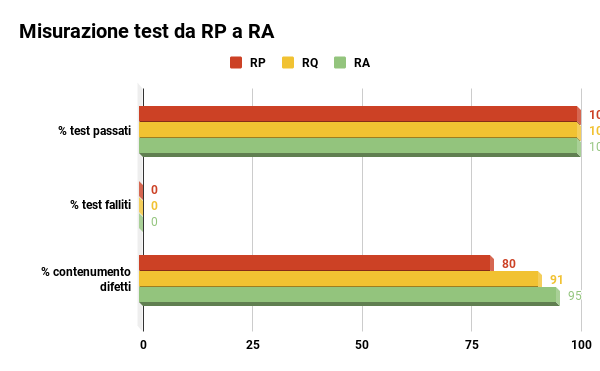
\includegraphics[width=13cm,keepaspectratio]{../includes/pics/MisurazioneRA.png}
	\caption{\label{fig:mission}MPRCS006 - Misurazione dei test da RP a RA}
\end{figure}
\pagebreak
\paragraph{MPRCS007 - Copertura requisiti}\mbox{}\\[0.4cm]
In questa revisione la copertura dei requisiti è pari al DA 94\%, valore considerato accettato per tale revisione.
\begin{figure}[H]
	\centering
	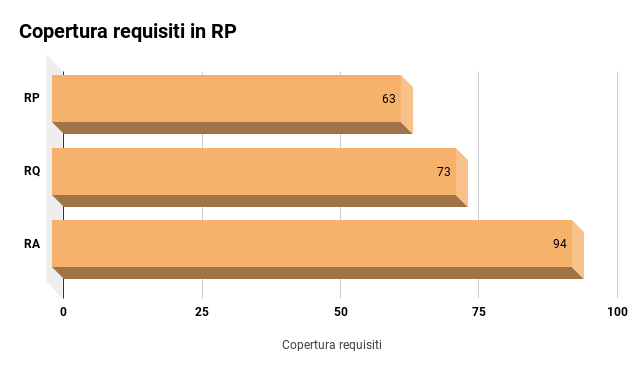
\includegraphics[width=13cm,keepaspectratio]{../includes/pics/CoperturaRP_RA.png}
	\caption{\label{fig:mission}MPRCS007 - Copertura}
\end{figure}
\paragraph{MPRDS014 - Code Coverage}\mbox{}\\[0.4cm]
\label{sec:CCRA}
In questa revisione il Code Coverage calcolato è pari al 98\%, valore considerato accettato per tale revisione.
\begin{figure}[H]
	\centering
	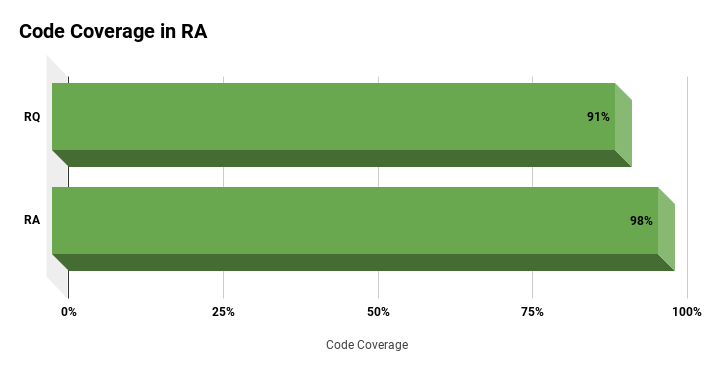
\includegraphics[width=13cm,keepaspectratio]{../includes/pics/ccRA.png}
	\caption{\label{fig:mission}MPRDS014 - Code Coverage}
\end{figure}